\documentclass[10pt,showpacs,preprintnumbers,footinbib,amsmath,amssymb,aps,prl,twocolumn,groupedaddress,superscriptaddress,showkeys]{revtex4-1}
\usepackage{graphicx}
\usepackage{dcolumn}
\usepackage{bm}
\usepackage[colorlinks=true,urlcolor=blue,citecolor=blue]{hyperref}
\usepackage{color}
\usepackage{amsmath}
\usepackage{multirow}
\usepackage{natbib}

\newcommand{\costa}[1]{% \costa{<power>}
	\ensuremath{\cos ^{#1} {\theta}} }
\newcommand{\sinta}[1]{% \sinta{<power>}
	\ensuremath{\sin ^{#1} {\theta}} }
\newcommand{\pwrten}[1]{%\pwrten{<power>}
	\ensuremath{10^{#1}} }
\newcommand{\rhomax}{
	\ensuremath{ \rho _{\mathrm{max}}} }
\newcommand{\fourpisqr}{
	\ensuremath{ 4 \pi ^2} }
\newcommand{\deriv}[3][]{% \deriv[<order>]{<function>}{<variable>}
	\ensuremath{ \frac{d ^{#1} {#2}}{d {#3}^{#1}}}}

\begin{document}
\title{PHY 905 Project 3: The Solar System}
\author{Thomas Redpath}
\affiliation{Department of Physics, Michigan State University, Outer Space}
\begin{abstract}
We present results from simulations of planetary dynamics involving two, three
and nine bodies. We demonstrate the stability of simulations utilizing the velocity
Verlet method over those using the Euler method. Using this algorithm, we find
that a three body Sun-Earth-Jupiter system with the Jupiter mass comparable
to $M _{\odot}$ results in a drastically altered Earth orbit whereas increasing
Jupiter's mass by a factor of 10 has no effect on the system. Finally, we
demonstrate the stability of all nine major bodies of the solar system over a
300 year period.
\end{abstract}
\maketitle

\section{Introduction}

The mathematical description of planetary motion via Newton's law
of gravitation is one of the great triumphs of classical physics. In this
report, we numerically solve Newton's equations using the velocity
Verlet method and model the dynamics of two and three body planetary
systems as well as the nine major bodies of the solar system. The
report is organized as follows: in the next section we give a brief summary
of the mathematical approach to solving Newton's equations and the
system of units used in this project. In the third
section we discuss the algorithms and methods we used, and in the fourth
section we present our results.


\section{Theory}

The familiar form for the gravitational force between the Earth and the Sun

\begin{equation}
	F_G=\frac{GM_{\odot}M_{\mathrm{Earth}}}{r^2},
	\label{eq:fgrav}
\end{equation}
gives the differential equation governing motion under the influence
of gravity:

\begin{equation}
	\deriv[2]{x_i}{t} = \frac{ F_{Gx_i}}{M_{\mathrm{Earth}}}
	\label{difeq}
\end{equation}
one for each directional coordinate $x_i$; so that $r^2 = \sum_i x_{i}^{2}$.
In this project, we will
model the solar system in three dimensions. Substituting the form
for $F_{Gx_i}$ (eq.~\ref{eq:fgrav}) and including a minus since the
force is attractive we obtain

\begin{equation*}
	\deriv[2]{x_i}{t} = - \frac{GM}{r^3} x_i
\end{equation*}
For our three dimensional case, there are three second order differential
equations which we can re-write as six first order differential equations.
These equations are coupled via $r^2 = \sum_i x_{i}^{2}$.

\begin{align*}
	\deriv[]{v_i}{t} &= - \frac{GM}{r^3}\\
	\deriv[]{x_i}{t} &= v_x
\end{align*}

\subsection*{Units}

We will work in astronomical units (AU for distance and years for time)
appropriate to the scale of this problem. Furthermore, we will use
mass ratios to the solar mass ($M _{\odot} = 2.0 \times \pwrten{30}$ kg).
With these units, the value for $GM_{\odot}$ is found to be $4\pi^2$ by
assuming circular orbits for which the angular acceleration is given by

\begin{align*}
	\frac{F_G}{M} &= \frac{v^2}{r} = \frac{G M_{\odot}}{r^2}\\
	v &= 2 \pi r \left [ \frac{\mathrm{AU}}{\mathrm{year}} \right ]\\
	& \Rightarrow v^2 r = GM_{\odot} = 4 \pi ^2 \left [ 
\frac{\mathrm{AU}^3}{\mathrm{year}^2} \right ]
\end{align*}

\section*{Algorithms and Methods}

The C++ code developed for this project primarily utilizes the velocity
Verlet method to solve the first order differential equations. For comparison,
we also coded and implemented Euler's method. In this section we briefly
summarize the derivations of these methods from \citet{Morten}. We
then provide a description of the codes which can be
found at \url{https://github.com/redpath11/phy905_thr} in the
\texttt{projects/project3} directory.

\subsection*{Euler's Method}

The first order differential equations may be solved numerically by
discretizing each dimension with a step size $h$. The numerical first
derivative for an arbitrary dimension $x$ comes from a Tayler
expansion

\begin{equation*}
	f _{i} = \frac{x _{i+1} - x{i}}{h} + O(h^2)
\end{equation*}
where $f$ is the first time derivative of $x$ (also a function of time)
and the subscripts denote time steps. The discretized position and velocity
equations for one dimension specialized to the gravitational case:

\begin{align*}
	x_{i+1} &= x_i + v_{i}h + O(h^2)\\
	v_{i+1} &= v_i - \frac{ \fourpisqr x_i }{r_i ^3 } h + O(h^2)
\end{align*}
where now $r_i$ is the magnitude of the radius vector at time step $i$.

\subsection*{Verlet Method}

The first order differential equations may also be solved using the
Verlet method which may be specialized to the graviational case
since the form of the acceleration is simple and known. The Verlet
method derives from a summation of two Taylor expansions. Consider
the position in one dimension

\begin{align*}
	x(t+h) &= x(t) + h x'(t) + \frac{1}{2} h^2  x''(t) + O(h^3)\\
	x(t-h) &= x(t)  - h x'(t) + \frac{1}{2} h^2  x''(t) + O(h^3).
\end{align*}
Summing these two expansions and switching to the discretized
notation gives

\begin{equation*}
	x_{i+1} = 2 x_i - x_{i-1} + h^2 x''_i + O(h^4).
\end{equation*}
In general, this algorithm is not self-starting since it requires the
value of $x$ at two previous points.

Now, consider a Taylor expansion of the velocity and note the
relationshipe between velocity and acceleration $v' = a$.

\begin{align*}
	v_{i+t} &= v_i + h v_i ' + \frac{1}{2} v_i '' + O(h^3)\\
	a_{i+1} &= v'_i + h v''_i + O(h^2).
\end{align*}
We will assume that the velocity is a linear function of time
$hv''_i \approx v'_{i+1} - v'_i$. We can now write the final
algorithmic form for the position and velocities.

\begin{align}
%%\begin{split}
	x_{i+1} &= x_i + hv_i + \frac{h^2}{2} v'_i + O(h^3)\\
	v_{i+1} &= v_i + \frac{h}{2}(v'_{i+1} + v'_i) + O(h^3)
\label{eq:Verlet}
%%\end{split}
\end{align}

\subsection*{Codes}

To test that we properly coded the algorithms, we first implemented them
in a simple C code (\texttt{src/p3test.cc}) using separate funcitons for the
Euler and Verlet methods to model the Sun-Earth system with the Sun fixed
at the center. We then expanded the code to implement the algorithms
within a class making it easier to add multiple planets to the simulation. We
modeled two classes after the examples provided by Morten Hjorth-Jensen
at \url{https://github.com/CompPhysics/ComputationalPhysicsMSU}. We
defined the first class to store the mass, position, velocity, kinetic and potential
energies of a planet in the simulation (see the \texttt{src/planet.cpp} file). The
second class (\texttt{src/ssystem.cpp}) holds an array of planet objects and
includes functions to implement the Euler and Verlet methods. These two
classes are used in the \texttt{p3main.cc} program to obtain the results
discussed in the next section.


\section{Results and discussion}

\subsection*{The Earth-Sun system}

First, we compare the Euler and velocity Verlet results for a simple two-body
system (the Sun and the Earth). For this comparison, we placed the sun at
the origin at rest and start the earth on the $y$ axis with an initial velocity
in the $-x$ direction and a magnitude given by the vector from \citep{nasa}.
We then adjust the step size in decades from 0.001 to 1. years. The results
are summarized in TABLE~\ref{tab:EVresults} and FIG.~\ref{fig:se001} - 
\ref{fig:se10}. In general, the Euler method is faster than the Verlet,
requiring only 4 floating point operations per step compared to the 6
operations per step needed by the Verlet algorithm. These estimates exclude
the operations necessary to compute the forces which are carried out in an
external function. The Verlet algorithm produces more stable results in terms
of energy and angular momentum. Physically, these quantities should be
conserved because there are no non-conservative forces and no external
torques acting on the system. Even with the 0.1 year step size, the
Verlet algorithm produces a semi-stable orbit (FIG.~\ref{fig:se1}), while
the Euler method gives orbits that spiral out even for the best step size
(FIG.~\ref{fig:se001}).

\begin{table}
\centering
	\begin{tabular}{ c | c c | c c c }
	Method & Step Size [yr] & Runtime [s] & $\Delta T$ & $\Delta U$ & $\Delta L$\\
\hline
	\multirow{4}{*}{Euler} & 0.001 & 1.2e-3 & 1.9e-5 & 7.7e-5 & -1.39\\
	                                     & 0.01   & 1.0e-4  & 3.1e-5 & 1.4e-4 & -4.36\\
	                                     & 0.1     & 1.3e-5  & 3.1e-5 & 2.3e-4 & -8.6\\
	                                      & 1.0     & 3e-6    & -2.3e-3 & 2.3e-4 & -2.9e2\\
\hline
	\multirow{4}{*}{Verlet} & 0.001 & 2.9e-3 & 7.4e-7 & 1.5e-6 & -5.3e-15 \\
	                                       & 0.01   & 3.0e-4 & 9.1e-7 & 1.8e-6 & -6.2e-15\\
	                                       & 0.1     & 3.0e-5 & 1.2e-5 & 2.6e-5 & 9.8e-15\\
	                                       & 1.0     & 4.0e-6 & -5.8e-4 & 2.4e-4 & -1.9e-14\\
\hline
	\end{tabular}
	\caption{Results of comparing the Euler and Verlet methods for the Sun-
	Earth system. The last three columns give the change (initial minus final)
	in the system kinetic energy, potential energy and angular momentum,
	respectively.}
	\label{tab:EVresults}
\end{table}



\subsection*{Escape Velocity}

We used our system and planet classes to determine the initial velocity needed
for a planet to escape the gravitational influence of the sun. To do this, we set
up a simple system with the Sun at rest at the origin and an arbitrary mass at 1
AU along $y$ with some initial velocity in the $-x$ direction. We calculated the
potential and kinetic energies for the planet, check the relationship KE $+$ PE
$< 0$ then incriment the starting velocity if this condition holds. We found that
an initial velocity of 8.9 AU/yr results in the planet's escape. This agrees with
the analytic result derived from the relationship mentioned earlier in this section:

\begin{align*}
	T + U &< 0\\
	\frac{1}{2} m v^2 &< \frac{ GM_{\odot} m}{r}\\
	v &< \sqrt{2GM_{\odot}/r}\\
	 &< \sqrt{8} \pi \approx 8.89, r=1 \mathrm{AU}
\end{align*}

\subsection*{The three body system}

Next, we modeled the three body Sun-Earth-Jupiter system and explored how
the third mass influences the planetary orbits. For this simulation, the Sun was
positioned at the origin at rest. The Earth and Jupiter were placed at 1 and 5.45
AU repectively along the $y$ axis. The planets' velocities were set according
to the magnitude of the velocity vectors obtained from \citep{nasa}. We tested
four different step sizes and found that for step sizes $\sim$ 1 year the discretization
becomes too crude to accurately model the system (see Table~\ref{tab:sejtest} and
the associated figures).

Next, we varied the Jovian mass to explore its effect on Earth's orbit. Using the
0.001 year step size, we ran our simulation with Jupiter's mass set to 10 and then 1000
times its actual value. The resulting orbits are shown in FIG.~\ref{fig:seJ10} and
FIG.~\ref{fig:seJ1000} where it is apparent that a Jupiter with roughly 1 solar mass would
force Earth into a collision with the Sun or eject it from the solar system in less than
20 years. For the $10M _J$ case, we ran our simulations for times up to 2000 years
and both orbits remained stable over this time.

We then included the motion of the sun about the three-body system's center
of mass. For this simulation, we calculated the total momentum of the Earth-
Jupiter system and gave the Sun a velocity to zero the total momentum of the
three body system; the resulting orbit is shown in FIG.~\ref{fig:sejfinal}. The
center of mass isn't perfectly stationary suggesting that the velocity we set for
the sun overcompensates for the planets' momenta and the whole system drifts
in the $+x$ direction. However, the simulated orbits are still stable.

\begin{figure}
\centering
	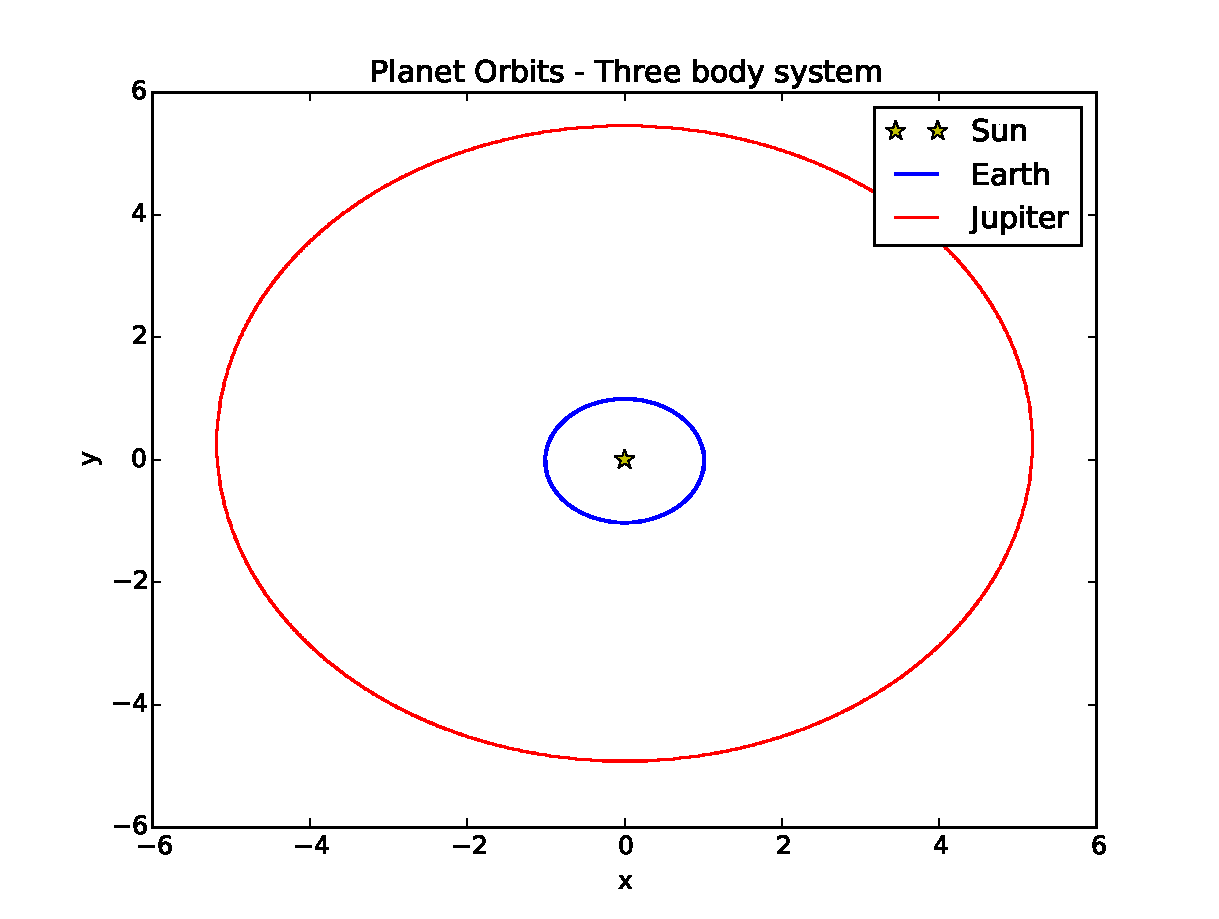
\includegraphics[width=0.5\textwidth]{figures/seJ10.pdf}
	\caption{Simulated three-body orbits with Jupiter's mass increased by a
	factor of 10.}
	\label{fig:seJ10}
\end{figure}

\begin{figure}
\centering
	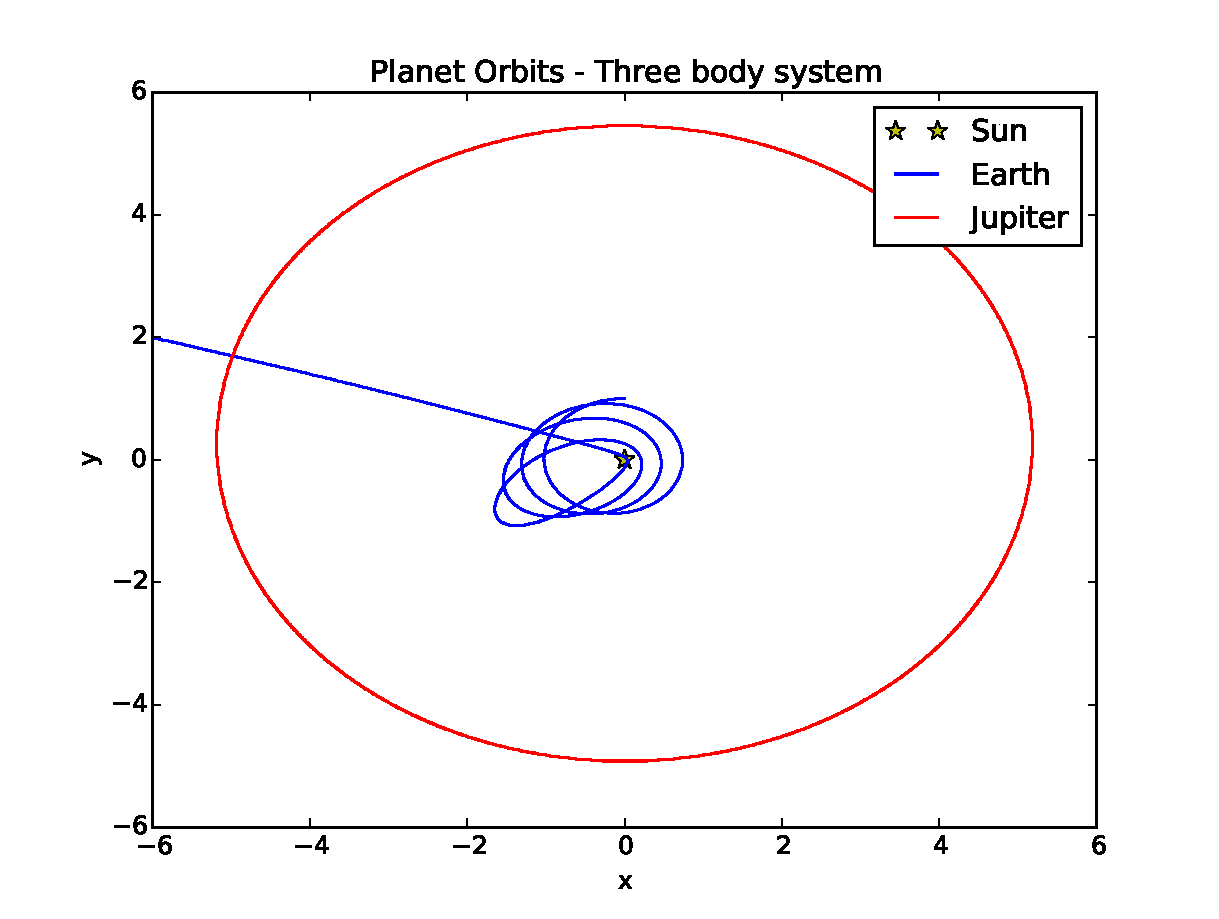
\includegraphics[width=0.5\textwidth]{figures/seJ1000.pdf}
	\caption{Simulated three-body orbits with Jupiter's mass increased by a
	factor of 1000.}
	\label{fig:seJ1000}
\end{figure}

\begin{figure}
\centering
	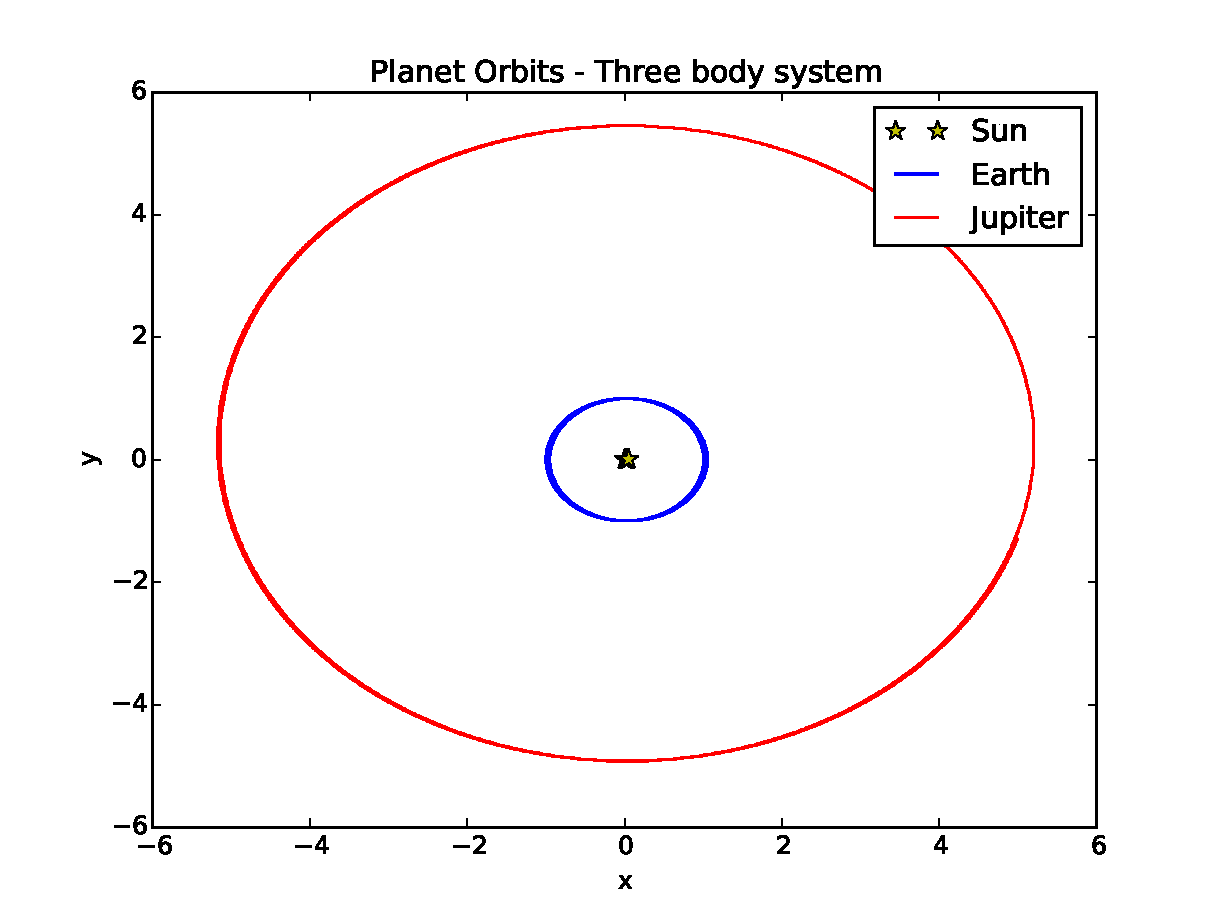
\includegraphics[width=0.5\textwidth]{figures/sejFinal.pdf}
	\caption{Simulated three-body orbits about the center of mass.}
	\label{fig:sejfinal}
\end{figure}

\begin{table}[h!]
\centering
	\begin{tabular}{ c c | c c c }
	Time [yr] & Step Size [yr] & Runtime [s] & Result & Figure\\
\hline
	20    & 0.001 & 0.019 & stable & \ref{fig:sej20}\\
	200   & 0.01 & 0.017 & stable & \ref{fig:sej200}\\
	2000 & 0.1 & 0.017 & stable & \ref{fig:sej2000}\\
	20000& 1.0& 0.032 & unstable & \ref{fig:sej20000}\\
\hline
	\end{tabular}
	\caption{Results of a stability test of the Verlet algorithm for the
	three body system. For each run, the number of steps is kept
	constant at 20000.}
	\label{tab:sejtest}
\end{table}



\subsection*{The solar system}

Finally, we simulated the full solar system with all nine planets over a period of 300
years, and a time step size of 0.001 years. We used the full position and velocity
vectors from \citep{nasa} to initialize the system and we ran the simulation for all
three dimensions. The resulting plots are separated according to the inner four and
outer five planets for ease of viewing (FIG.~\ref{fig:ssi}, FIG.~\ref{fig:sso}).

\subsection*{Precession of the Perihelion of Mercury}

We specialized our Verlet algorithm for the Mercury-Sun system to study the
precession of the perihelion of Mercury's orbit. This observed precession was
unable to be accounted for by purely Newtonian effects. It was not until Einstein
formulated General Relativity and applied it to this problem that the $43''$ per
century discrepancy between the Newtonian predicted precession and the
observed precession was resolved.

In our attempt to model this phenomenon, we included a relativistic correction
to the gravitational force

\begin{equation*}
F_G = \frac{GM_\mathrm{Sun}M_\mathrm{Mercury}}{r^2}\left[1 + \frac{3l^2}{r^2c^2}\right]
\end{equation*}
and ran a simulation of the Mercury-Sun system over 100 years starting Mercury at perihelion
and placing the Sun at the origin at rest. In order to select the proper time
step size, we ran a series of simulations without the relativistic correction, decrimenting
the time step size until the perihelion precession was $\sim \pwrten{-4}$ after a century.
This occurred for $\Delta t = \pwrten{-6}$ (see \texttt{Benchmark/NoHgPrecess.out}.
We then added the relativistic correction and observed a precession of 0.25 degrees over
100 years (see \texttt{Benchmark/HePrecess.out} - this is roughly 20 times $43''$.
Unfortunately, we were unable to find the source of this error.



\begin{figure}
\centering
	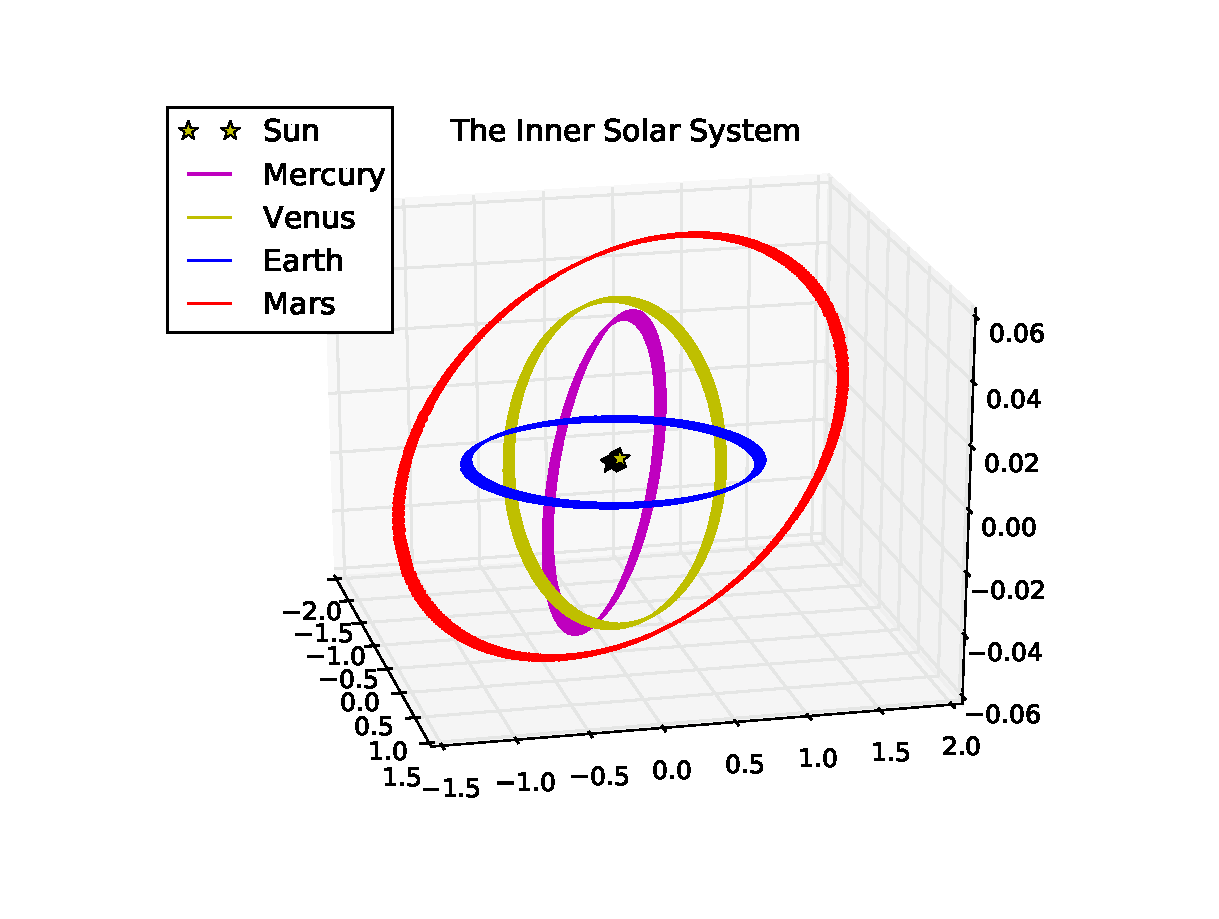
\includegraphics[width=0.5\textwidth]{figures/SSinner.pdf}
	\caption{The inner solar system.}
	\label{fig:ssi}
\end{figure}

\begin{figure}
\centering
	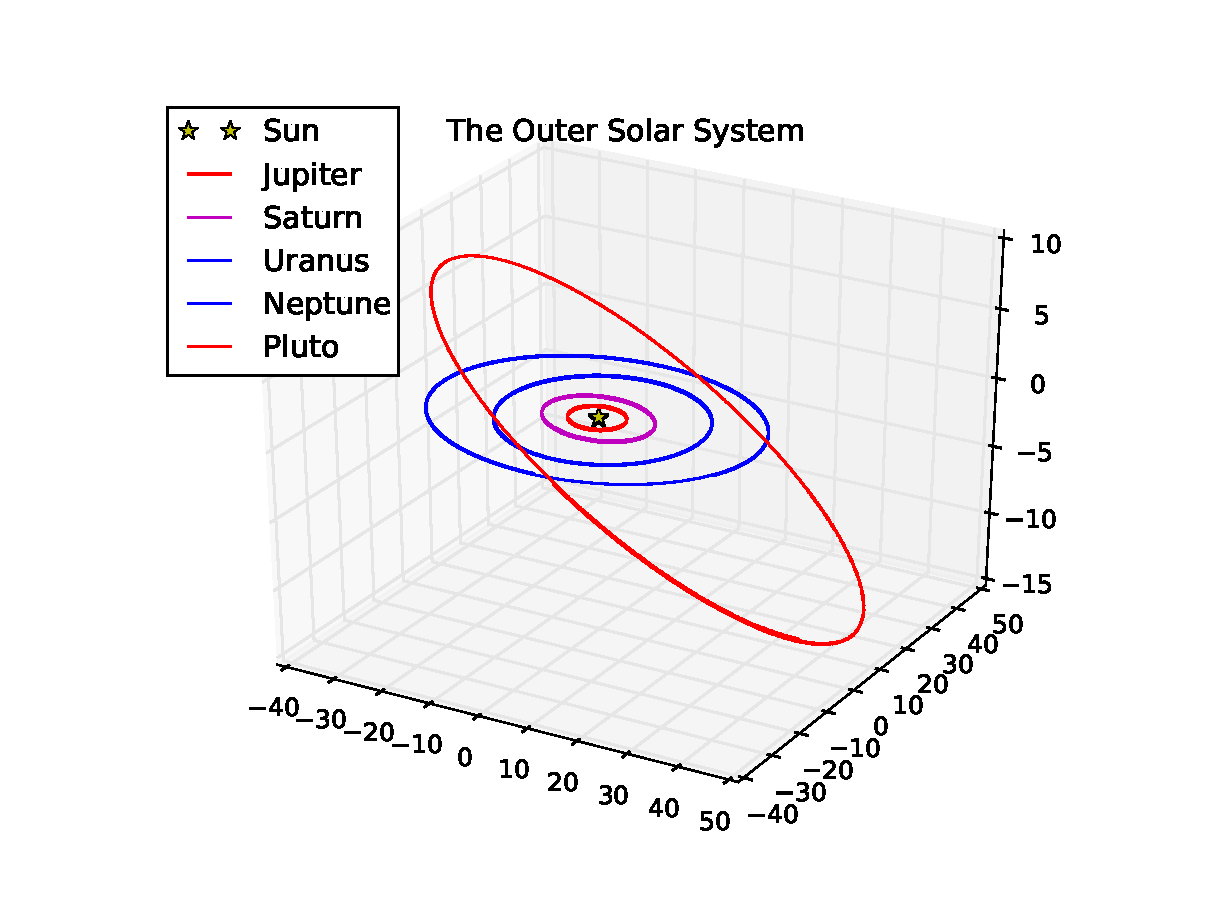
\includegraphics[width=0.5\textwidth]{figures/SSouter.pdf}
	\caption{The outer solar system.}
	\label{fig:sso}
\end{figure}

%\begin{figure}
%\centering
%	\includegraphics[width=0.5\textwidth]{figures/dnit2.pdf}
%	\caption{The number of similarity transformations needed to
%	diagonalize the matrix is plotted against the matrix
%	dimensionality. A quadratic fit gives a $2 N^2 - 8 N$ dependence
%	of the number of similarity transformations on the dimensionality
%	$N$.}
%	\label{fig:dnit}
%\end{figure}


%\begin{figure}
%\centering
%	\includegraphics[width=0.5\textwidth]{figures/gsw.pdf}
%	\caption{Ground state wavefunctions for different oscillator
%	strengths and no interaction between the electrons.
%	The weakest potential ($\omega = 0.01$) is shown in black and the
%	strongest potential ($\omega = 5$) is plotted in green.
%	The wavefunctions have been scaled to the $\omega = 5$ wavefunction.}
%	\label{fig:gsw}
%\end{figure}

%\begin{figure}[hbtp]
%\includegraphics[scale=0.4]{test1.pdf}
%\caption{Exact and numerial solutions for $n=10$ mesh points.} 
%\label{fig:n10points}
%\end{figure}



%\begin{figure}[h!]
%\centering
%	\includegraphics[width=0.5\textwidth]{figures/CIwvfn.pdf}
%	\caption{Ground state wavefunctions vs. separation distance for two
%	Coulomb-interacting electrons in a harmonic oscillator potential.}
%	\label{fig:ci}
%\end{figure}

\section{Conclusions}

We have applied Euler's method and the velocity Verlet algorithm to
model the gravitational interaction of planetary bodies. We developed
two C++ classes to run these simulations. In a comparison of the two
algorithms, we found that the Verlet method produces stable
orbits and gives a better approximation to energy and angular momentum
conservation than Euler's method. We tested our Verlet code by
simulating the orbital dynamics for a two-body Earth-Sun system
and a three body Earth-Jupiter-Sun system. We found that a step size
of 0.001 years is sufficient to model these systems over a 20 year period.
We also studied the effect of increasing Jupiters mass on the Earth's orbit
for the three body system. We found that Earth's orbit is severely altered
for a Jupiter mass $\sim 1 M_{\odot}$. Finally, we simulated the full solar
system in three dimensions over a 300 year period including gravitational
interactions between all the planets.

%\begin{thebibliography}{99}
%%\bibitem{miller2006} G.~A.~Miller, A.~K.~Opper, and E.~J.~Stephenson, Annu.~Rev.~Nucl.~Sci.~{\bf 56}, 253 (2006).
%\end{thebibliography}

\clearpage

%\section*{Figures}

\begin{figure}
\centering
	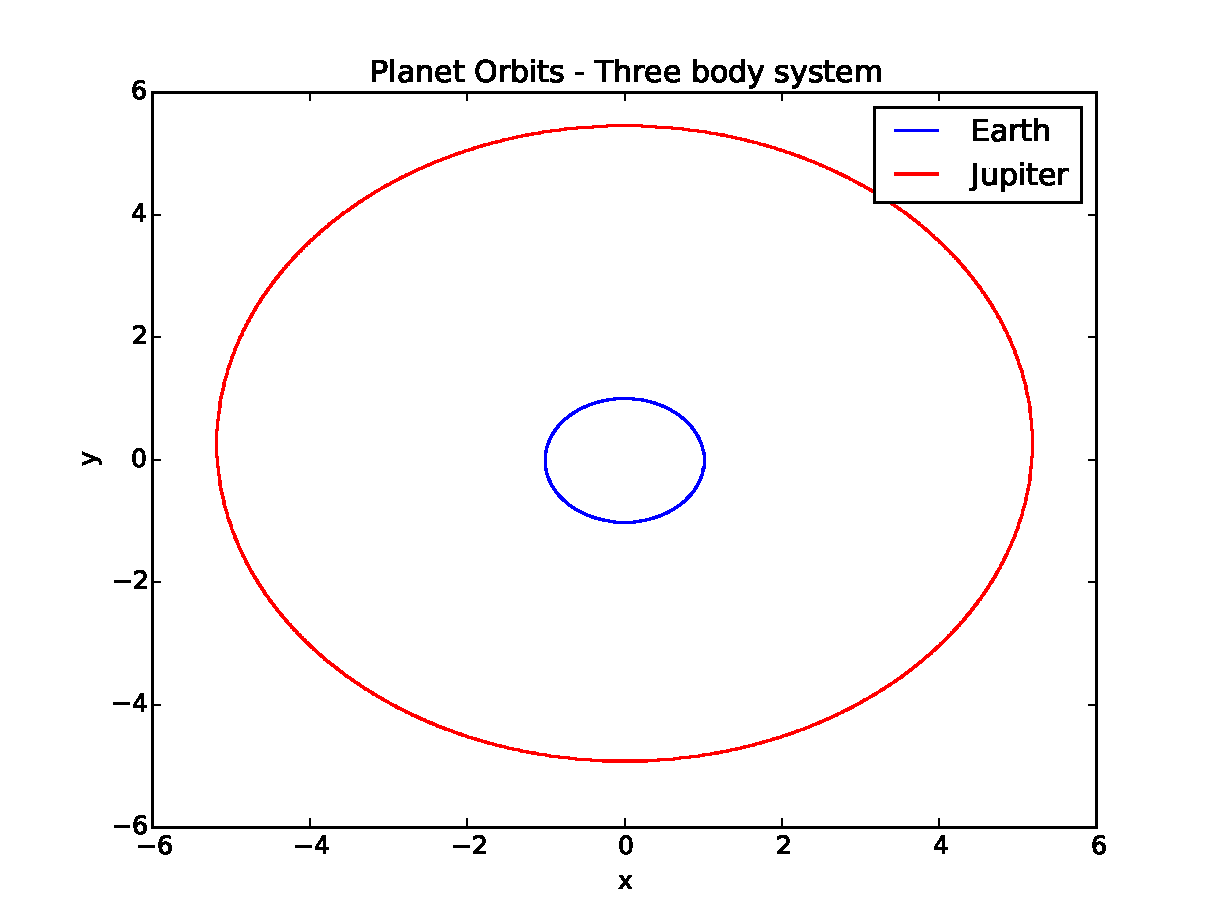
\includegraphics[width=0.5\textwidth]{figures/sej20.pdf}
	\caption{Earth and Jupiter orbits produced in the three-body
	simulation with a 0.001 years step size. We note that this
	same plot is produced regardless of the final time as long
	as number of steps is set such that the step size is 0.001 years
	and the final time is chosen
	to be longer than one Jovian orbital period (11.86 years).}
	\label{fig:sej20}
\end{figure}

\begin{figure}
\centering
	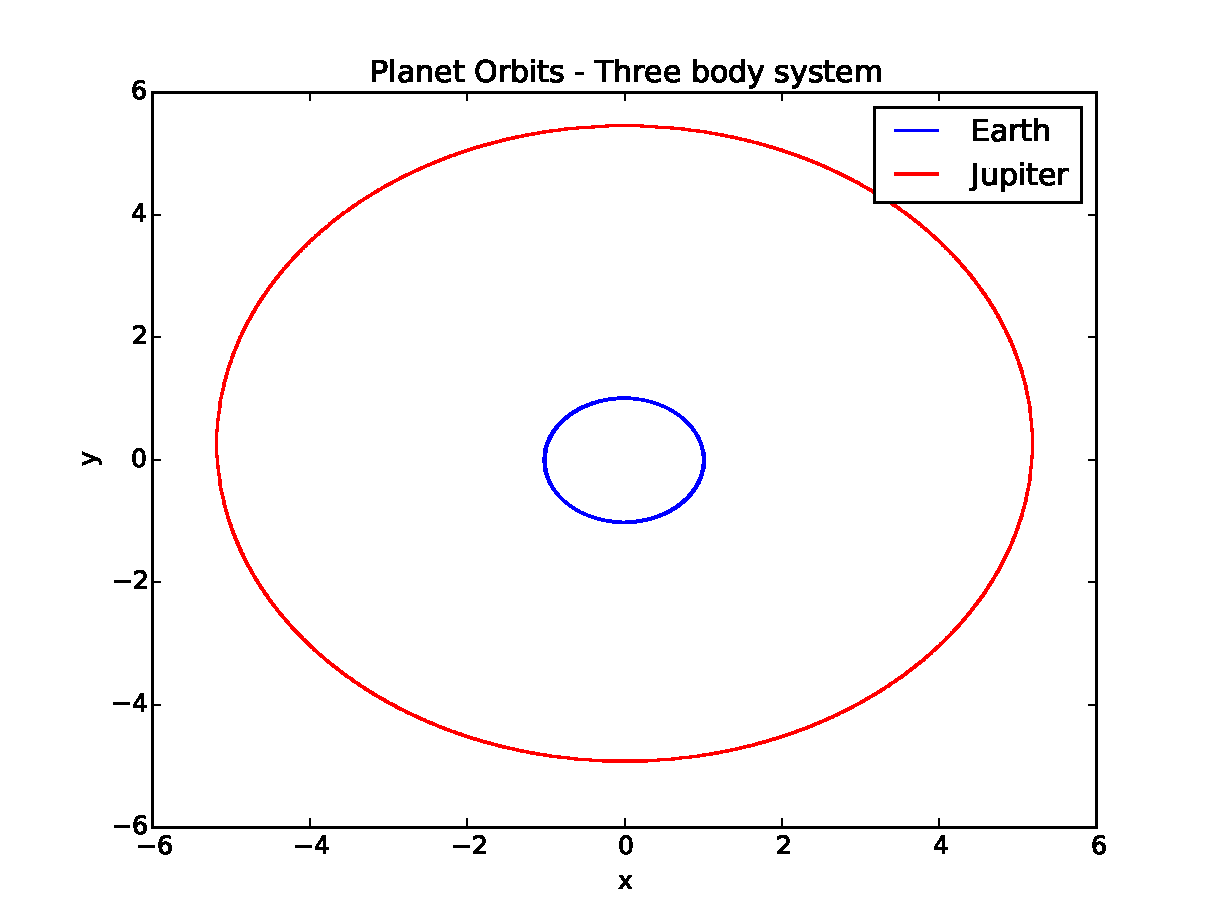
\includegraphics[width=0.5\textwidth]{figures/sej200.pdf}
	\caption{Earth and Jupiter orbits produced in the three-body
	simulation with a 0.01 years step size.}
	\label{fig:sej200}
\end{figure}

\begin{figure}
\centering
	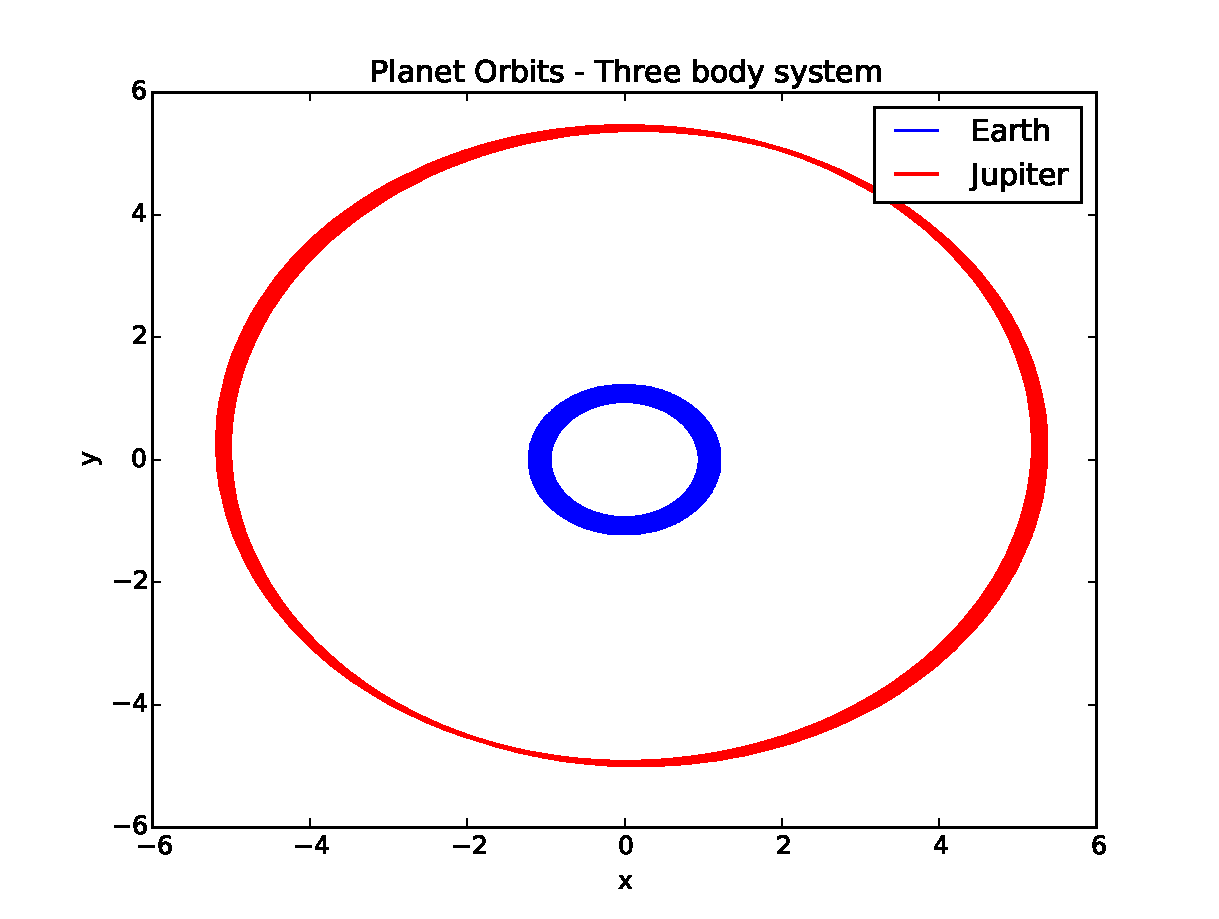
\includegraphics[width=0.5\textwidth]{figures/sej2000.pdf}
	\caption{Earth and Jupiter orbits produced in the three-body
	simulation with a 0.1 years step size.}
	\label{fig:sej2000}
\end{figure}

\begin{figure}
\centering
	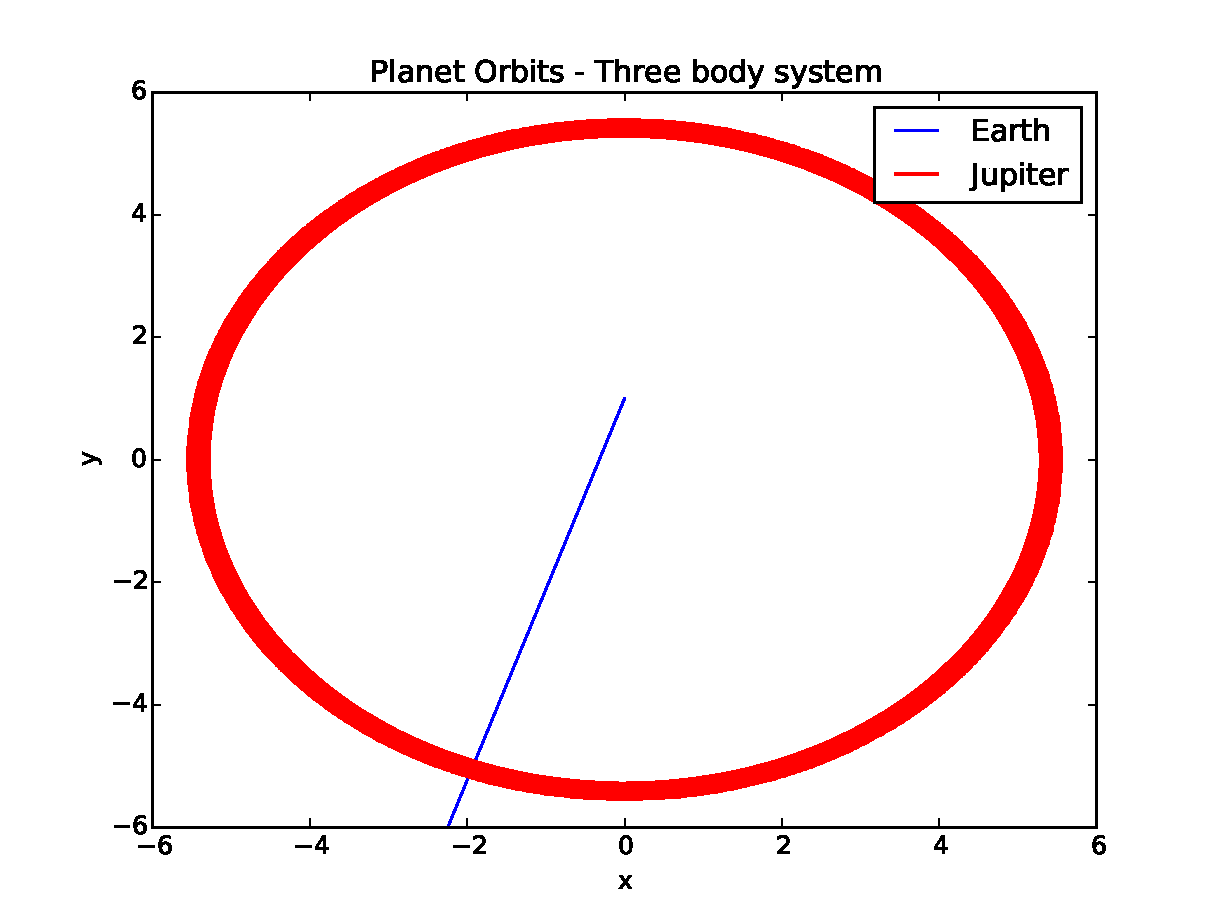
\includegraphics[width=0.5\textwidth]{figures/sej20000.pdf}
	\caption{Earth and Jupiter orbits produced in the three-body
	simulation with a 1 year step size.}
	\label{fig:sej20000}
\end{figure}

\clearpage

\begin{figure}
\centering
	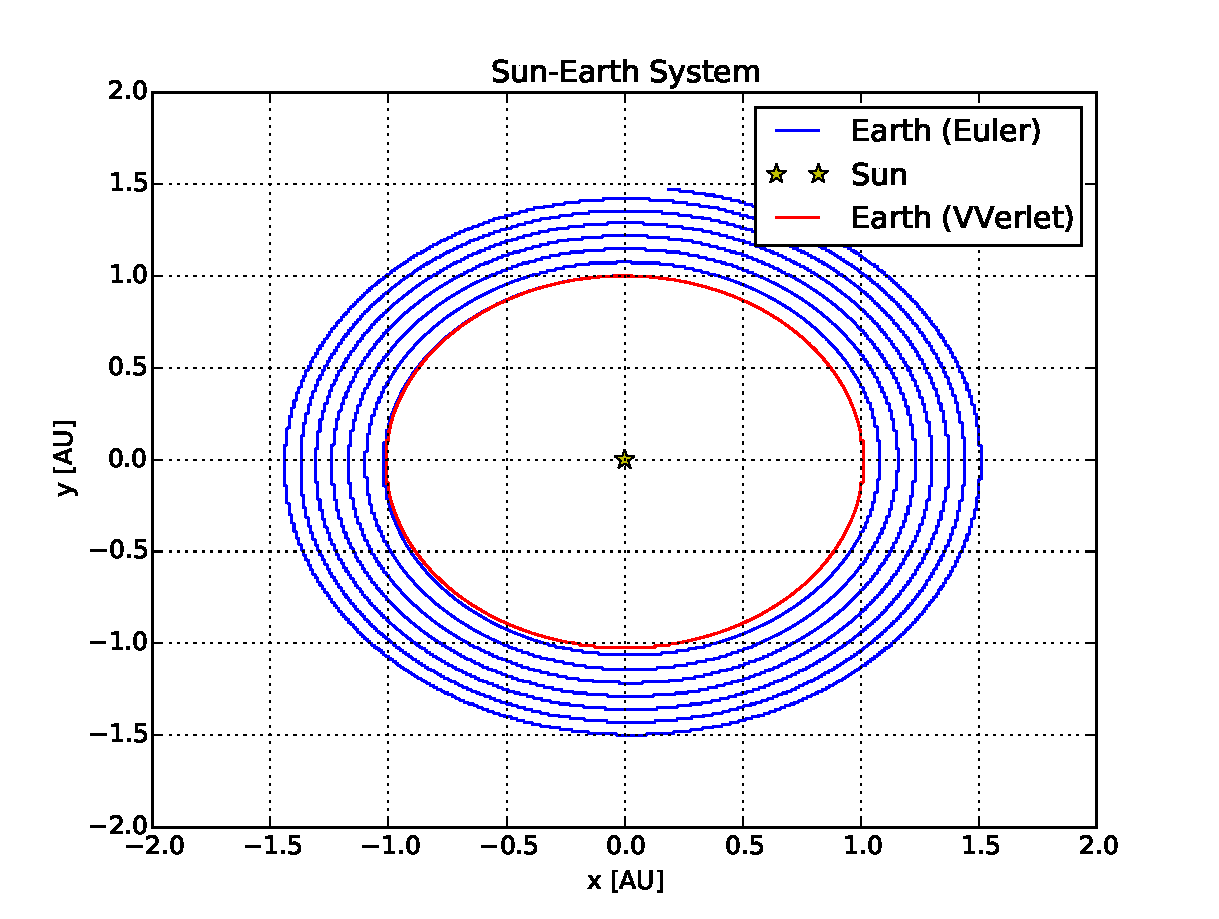
\includegraphics[width=0.5\textwidth]{figures/se001.pdf}
	\caption{Simulated Earth orbits over 10 years using the Euler (blue) and
	Verlet (red) methods. The time step size is 0.001 years.}
	\label{fig:se001}
\end{figure}

\begin{figure}
\centering
	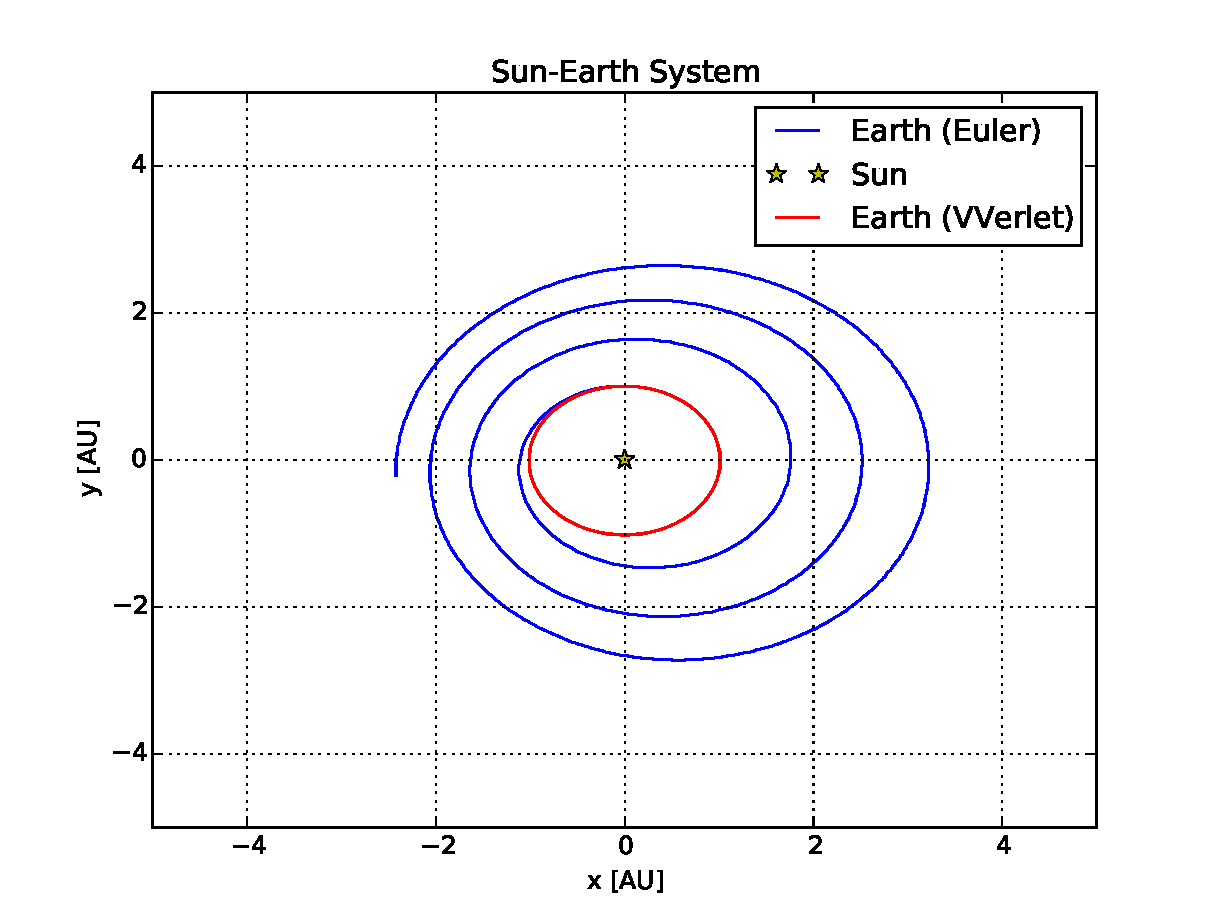
\includegraphics[width=0.5\textwidth]{figures/se01.pdf}
	\caption{Simulated Earth orbits over 10 years using the Euler (blue) and
	Verlet (red) methods. The time step size is 0.01 years.}
	\label{fig:se01}
\end{figure}

\begin{figure}
\centering
	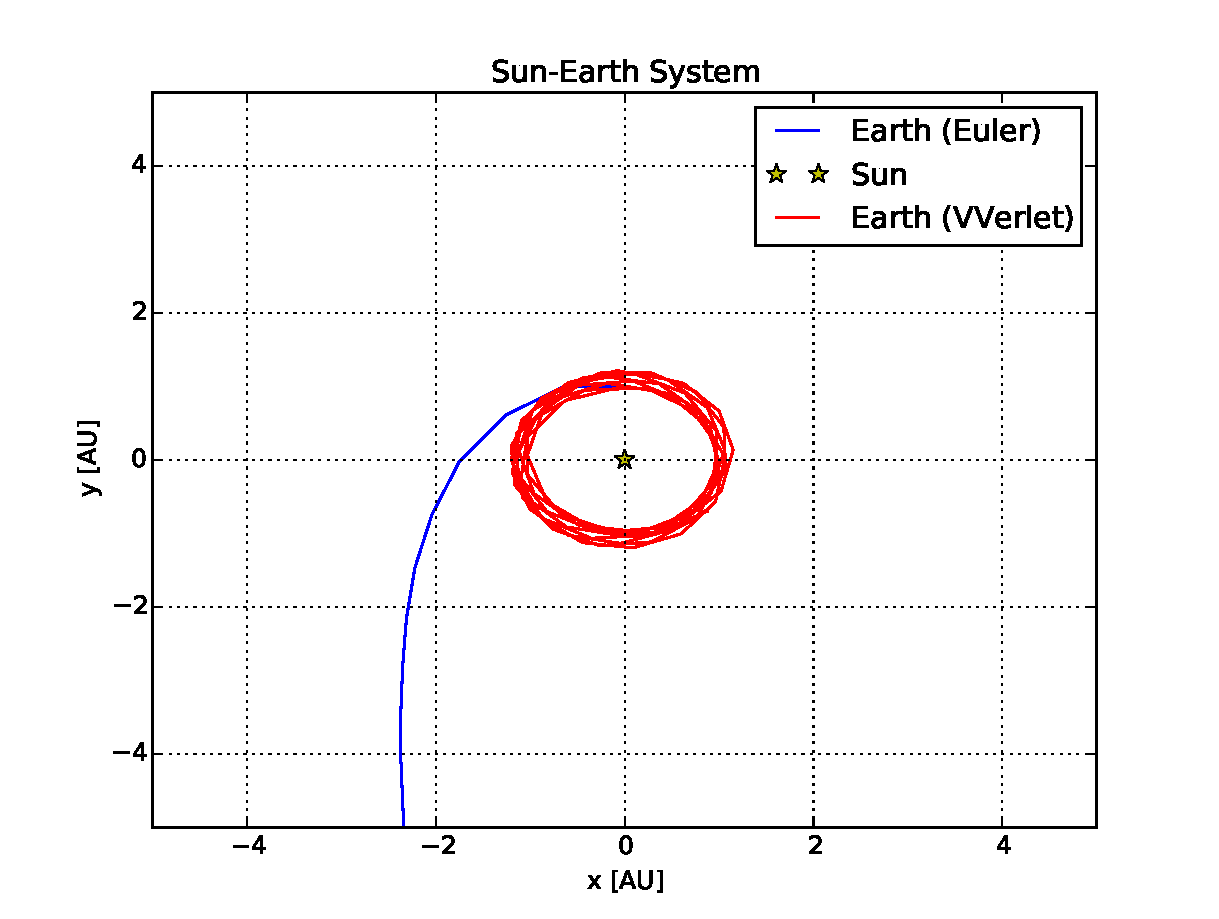
\includegraphics[width=0.5\textwidth]{figures/se1.pdf}
	\caption{Simulated Earth orbits over 10 years using the Euler (blue) and
	Verlet (red) methods. The time step size is 0.1 years.}
	\label{fig:se1}
\end{figure}

\begin{figure}
\centering
	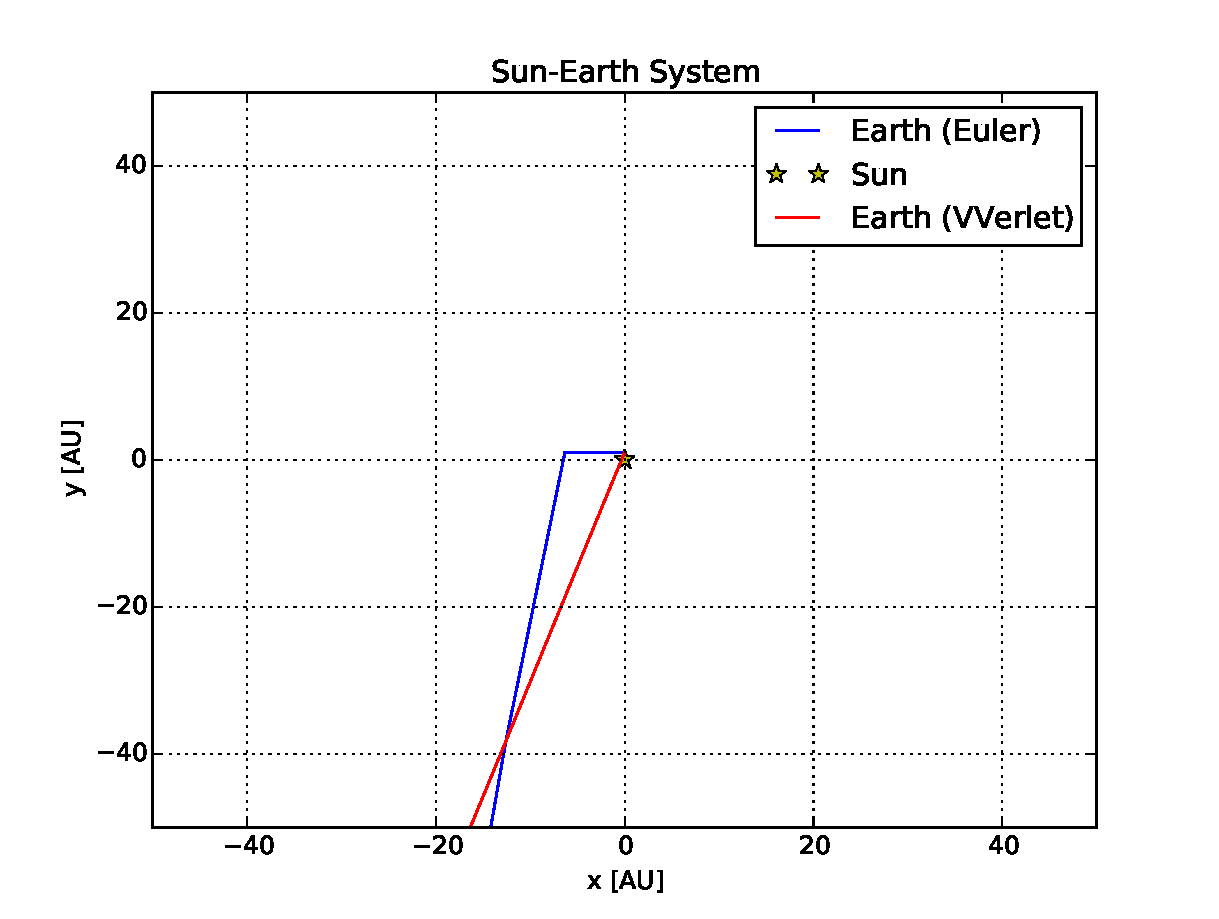
\includegraphics[width=0.5\textwidth]{figures/se10.pdf}
	\caption{Simulated Earth orbits over 10 years using the Euler (blue) and
	Verlet (red) methods. The time step size is 1 year.}
	\label{fig:se10}
\end{figure}

\clearpage

\bibliographystyle{plainnat}
\bibliography{refs}

\end{document}